\documentclass[11pt]{beamer}
\usetheme{Warsaw}
\usepackage[utf8]{inputenc}
\usepackage[brazil]{babel}  % idioma
\usepackage{amsmath,amsfonts,amssymb,textcomp}
\usepackage{graphicx}
\usepackage{subfigure}

% Configurando layout para mostrar codigos C++
\usepackage{listings}
%\usepackage{minted}
%pdflatex -shell-escape minted01.tex
%ou
%latexmk -pdf -shell-escape minted01.tex

\author{Othon Oliveira}
\title{Sistemas Operacionais}
%\setbeamercovered{transparent} 
%\setbeamertemplate{navigation symbols}{} 
%\logo{} 
\institute{Fatec -- Faculdade de Informática --- PE} 
%\date{} 
%\subject{} 
\begin{document}


% Capa - requer o TikZ
\newcommand{\capa}{
    \begin{tikzpicture}[remember picture,overlay]
        \node at (current page.south west)
            {\begin{tikzpicture}[remember picture, overlay]
                \fill[shading=radial,top color=orange,bottom color=orange,middle color=yellow] (0,0) rectangle (\paperwidth,\paperheight);
            \end{tikzpicture}
          };
    \end{tikzpicture}
}




\begin{frame}
\titlepage
\end{frame}

\begin{frame}
\tableofcontents
\end{frame}



%+++++++++++++++++++++++++++++++++++++++++++++++
\section{Threads}
\subsection*{Conceito -- revisão}

\begin{frame}{Espaço de endereçamento}
 Em sistemas tradicionais, cada processo tem um espaço de endereçamento e um único Thread (fluxo) de controle.
 
\pause
 \begin{block}{Definição}
 	Isso é quase uma definição de processo, exceto pelo espaço de endereçamento
 \end{block}
 
 \pause
 Contudo é frequente querer ter múltiplos threads em um único espaço de endereçamento executando em quase-paralelamente, como se fossem processos separados.
\end{frame}


%+++++++++++++++++++++++++++++++++++++++++++++++
\begin{frame}\frametitle{ Exemplo}

\begin{block}{ Um servidor Web}
Um modo de organizar o servidor Web é mostrado na figura acima.
Na figura, um thread, o \textbf{despachante}, lê as requisições que chegam à rede. 
Depois de examinar a requisição, ele escolhe um thread \textbf{operário} ocioso (isto é bloqueado) e entrega-lhe a requisição, 
possivelmente com um ponteiro associado a mensagem e uma palavra especial para cada thread. 
Na prática o despachante ``acorda'' o operário que está descansando, tirando-o do estado bloqueado e colocando-o no estado pronto.
\end{block}

\end{frame}

%+++++++++++++++++++++++++++++++++++++++++++++++
\begin{frame}{ Um servidor Web}
\begin{figure}[h]

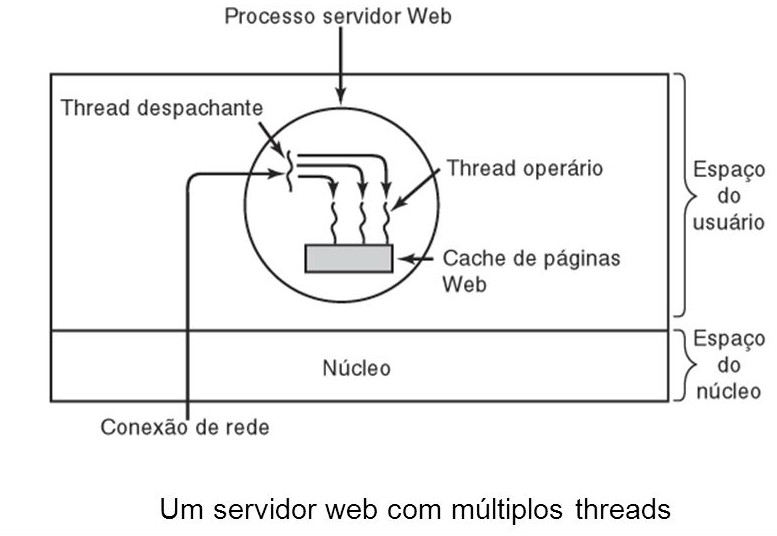
\includegraphics[width=100mm, height=60mm]{Figuras/threadsServidor.jpg}
\end{figure}

\end{frame}



%+++++++++++++++++++++++++++++++++++++++++++++++
\defverbatim[colored]\lstDsp{
\begin{lstlisting}[language=C++,basicstyle=\ttfamily\small,keywordstyle=\color{blue},stringstyle=\color{verde},commentstyle=\color{red}, 
  extendedchars=true,showspaces=false,showstringspaces=false,numbers=left,numberstyle=\tiny,breaklines=true,backgroundcolor=\color{green!10},
  breakautoindent=true,captionpos=b,xleftmargin=0pt]
while(true){\\
  // Uma implementacao da figura anterior
  // um bloco, em C:
  get_next_request(&buf);\\
  handoff_work(&buf);\\
}
\end{lstlisting}
}

\begin{frame}{ Thread Despachante}{C,C++}
\lstDsp
\end{frame}

%+++++++++++++++++++++++++++++++++++++++++++++++
\defverbatim[colored]
\lstOp{
\begin{lstlisting}[language=C++,basicstyle=\ttfamily\small,keywordstyle=\color{blue},stringstyle=\color{verde},commentstyle=\color{red}, 
  extendedchars=true,showspaces=false,showstringspaces=false,numbers=left,numberstyle=\tiny,breaklines=true,backgroundcolor=\color{green!10},
  breakautoindent=true,captionpos=b,xleftmargin=0pt]
while(true){
  wait_for_work(&buf);
  look_for_page_in_cache(&buf, &page);
  if(page_not_in_cache(&page)) read_page_from_disk(&buf, &page);
  return_page(&page);
}
\end{lstlisting}
}

\begin{frame}{ Thread Operário}{C,C++}
\lstOp 
\pause

\begin{block}{ Pergunta}
 Este exemplo é multithreads ou monothread ??
\end{block}
\end{frame}


%+++++++++++++++++++++++++++++++++++++++++++++++
\begin{frame}\frametitle{ Explicando o código}

\begin{block}{ Um servidor Web}
Esse modelo permite que o servidor seja escrito como uma coleção de threads sequenciais.
O programa do despachante consiste num laço infinito para obter requisições de trabalho e entregá-las a um operário.
Cada código de operário consiste em um laço infinito que acata uma requisição de um despachante e verifica se a página está presente na cache 
de páginas Web. Se estiver, entrega-a ao cliente e bloqueia esperando uma nova requisição.
\end{block}

\pause
\begin{block}{ monothread}
 Porém o código anterior é monothread
\end{block}

\end{frame}


%+++++++++++++++++++++++++++++++++++++++++++++++
\section{Implementação de threads}
\subsection*{Implementação de threads de usuários}

\begin{frame}{Espaço do Usuário}
 Há muitos de implementar um pacote de threads: no espaço do usuário e no núcleo.
 Essa escolha é um pouco controversa. Exite também a implementação híbrida.
 \begin{block}{ Thread de usuário}
  O primeiro método é inserir o pacote de threads totalmente dentro do espaço do usuário (threads de usuário).
  O núcleo não é inforamdo sobre eles. O que compete ao núcleo é gerir os processos.
 \end{block}
 
\end{frame}


%+++++++++++++++++++++++++++++++++++++++++++++++
\begin{frame}{ Thread de usuário}
\begin{figure}[h]

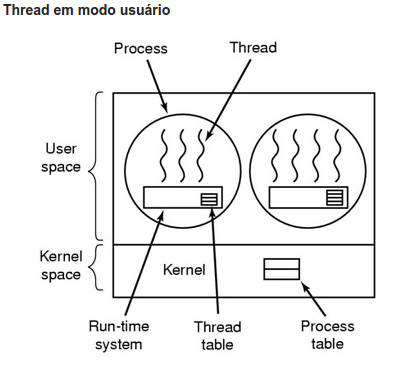
\includegraphics[width=100mm, height=60mm]{Figuras/threadusuario}
\end{figure}

\end{frame}

%+++++++++++++++++++++++++++++++++++++++++++++++
\subsection*{Implementação de threads de núcleo}

\begin{frame}{Espaço do kernel}
 Considere que o núcleo saiba sobre os threads e os gerencie.
 Não é necessário um sistema de supervisor como mostrado na figura anterior
 
 \pause
 \begin{block}{Definição}
  Não há também uma tabela de threads em cada processo.
  Em vez disso o núcleo tem uma tabela de threads que acompanha todos os threads do sistema.
 \end{block}
 
  \pause
  \begin{block}{Definição}
  Quando um thread que criar um novo thread ou destruir um já existente, faz uma chamada ao núcleo, que realiza então a criação ou a destruição 
  atualizando a tabela de threads do núcleo.
 \end{block}
\end{frame}


%+++++++++++++++++++++++++++++++++++++++++++++++
\begin{frame}{ Threads de núcleo -- kernel}
\begin{figure}[h]

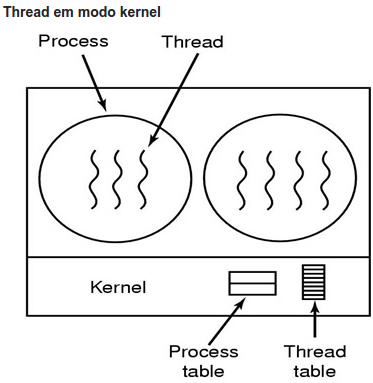
\includegraphics[width=100mm, height=60mm]{Figuras/threadnucleo}
\end{figure}

\end{frame}

%+++++++++++++++++++++++++++++++++++++++++++++++
\subsection*{Implementação de threads de hibridas}

\begin{frame}{ Threads híbridas}
 Vários modos de tentar combinar as vantagens dos threads de usuário com os threads de núcleo têm sido investigados.
 
 \pause
 \begin{block}{Multiplexar threads}
 Um deles é usar threads de núcleo e então Multiplexar threads de usuários sobre algum ou todos os threads de núcleo.
 \end{block}
 
\end{frame}

%+++++++++++++++++++++++++++++++++++++++++++++++
\begin{frame}{ Threads híbridas}
\begin{figure}[h]

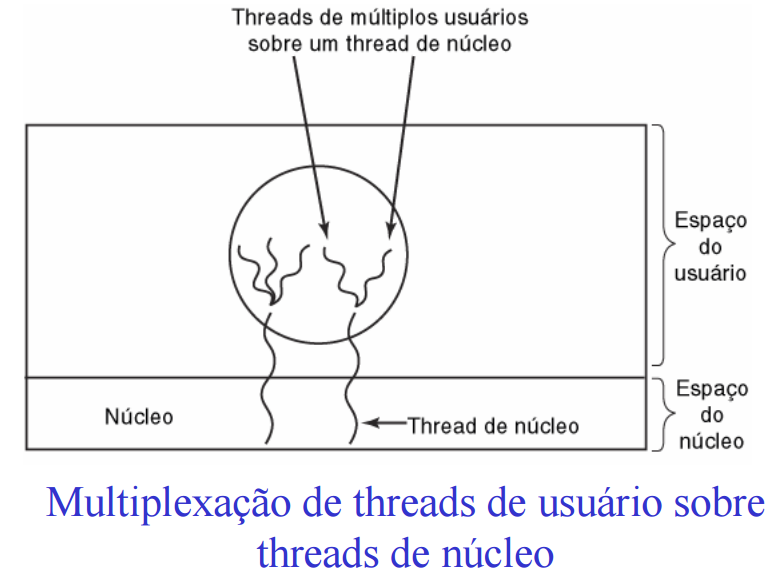
\includegraphics[width=100mm, height=60mm]{Figuras/threadhibrida}
\end{figure}

\end{frame}


%+++++++++++++++++++++++++++++++++++++++++++++++
\section{Comunicação entre processos}
\subsection*{Introdução}

\begin{frame}{ A Comunicação entre processos}
 Em um pipeline do interpretador de comandos, a saída do primeiro processo deve ser passada para o segundo processo, e isso prossegue até o 
 fim da linha de comando. Assim há uma necessidade de comunicação entre processos
\pause
 \begin{block}{Tipos}
 \begin{itemize}
  \item Condição de disputa
  \pause
  \item Regiões críticas
  \pause
  \item Exclusão mútua com espera ociosa
  \pause
  \item Dormir e acordar
  \pause
  \item Semáforos
  \pause
  \item Mutexes
  \pause
  \item Monitores
 \end{itemize}
 \end{block}
  
\end{frame}


%+++++++++++++++++++++++++++++++++++++++++++++++
\subsection*{Condição de disputa}
\begin{frame}
  Em alguns sistemas operacionais, processos que trabalham juntos podem compartilhar algum armazenamento comum.
  A seguir dois processos tentar escrever arquivos na fila de impressão
 \begin{figure}[h]
  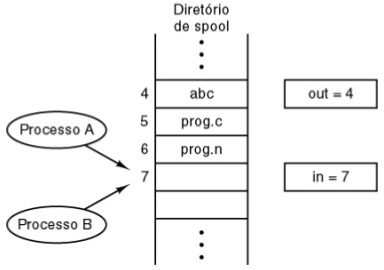
\includegraphics[width=80mm, height=40mm]{Figuras/disputa}
  \end{figure}

\end{frame}

%+++++++++++++++++++++++++++++++++++++++++++++++
\subsection*{Regiões críticas}
  
\begin{frame}{ O que fazer para evitar condições de disputa? Exclusão mútua}
 A resposta para evitar disputa em memória compartilhada é evitar de alguma maneira que processos leiam e escrevam ao mesmo tempo na memória 
 compartilhada.
 \begin{block}{ Região de Exclusão}
 Em outras palavras uma maneira de assegurar que outros processos sejam impedidos de usar uma variável ou um arquivo compartilhado 
 que já estiver em uso por outro processo é criar uma Região de Exclusão.
 \end{block}

\end{frame}

\begin{frame}{ Isso é suficiente??}
 Embora essa solução impeça as condições de disputa, isso não é suficiente
 Precisamos satisfazer quatro condições
 \begin{block}{ Região Críticas}
 \begin{itemize}
  \item Nunca dois processos podem estar simultaneamente em suas regiões críticas.
  \pause
  \item Nada pode ser afirmado sobre a velocidade ou sobre o número de CPUs.
  \pause
  \item Nenhum processo executando fora da região crítica pode bloquear outros processos.
  \pause
  \item Nenhum processo deve esperar eternamente para entrar em sua região crítica.
 \end{itemize}
 \end{block}

\end{frame}

%+++++++++++++++++++++++++++++++++++++++++++++++
\subsection*{ Regiões Críticas}
\begin{frame}{ Exclusão mútua usando Regiões Críticas}
  
 \begin{figure}[h]
  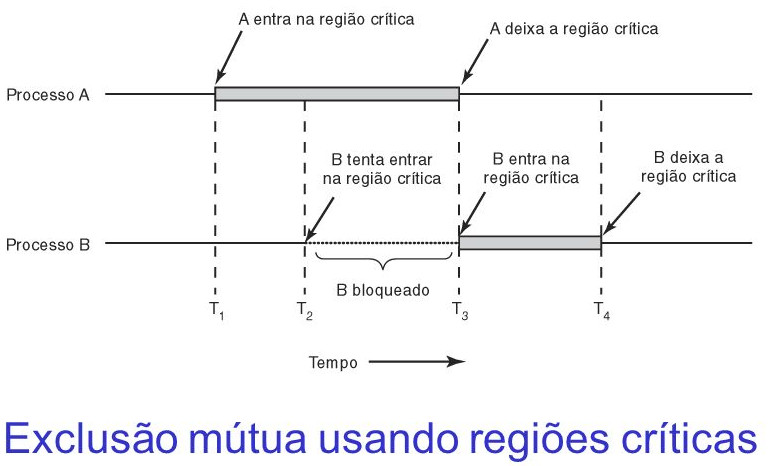
\includegraphics[width=80mm, height=40mm]{Figuras/exlcusaomutua}
  \end{figure}

\end{frame}

%+++++++++++++++++++++++++++++++++++++++++++++++
\subsection{Exclusão mútua com espera}

\begin{frame}{Desabilitando interrupções}
 Estudaremos várias alternativas para realizar Exclusão Mútua de modo que nenhum outro processo invada a região de memória compartilhada.
 \begin{block}{Desabilitando interrupções da CPU}
 A solução simples é aquela que cada processo desabilita todas as interrupções logo depois de entrar em sua região crítica e reabilita-as 
 antes de sair dela.
 \end{block}
 
 \pause
 \begin{block}{Desabilitando interrupções da CPU}
 Pode ser necessário o próprio núcleo desabilitar as interrupções, para umas poucas instruções enquanto estiver alterando Variáveis ou listas.
 \end{block}
\end{frame}

%-------------------------------------------
\begin{frame}{Variáveis de impedimento(lock variables)}
 Uma solução por software
 
 \pause
  \begin{block}{Definição}
 Para entrar em sua região crítica, um processo testa antes se a variável \textit{lock} é zero (0) o processo altera altera para 1 e entra 
 na região crítica. Infelizmente essa técnica apresenta a mesma falha que vimos no diretório de spool.
  \end{block}
 
 Caso outro processo ao mesmo tempo leia a variável \textit{lock} alterando para 1 haverão 2 processos em suas Regiões Críticas.
\end{frame}

%-------------------------------------------
\begin{frame}{Alternância obrigatória}

 \begin{block}{ Pesquisa}
 \begin{itemize}
  \item Pesquisar sobre Alternância obrigatória
  \pause
  \item Solução de Paterson
  \pause
  \item A instrução TSL
 \end{itemize}

  
 \end{block}
 
\end{frame}

%-------------------------------------------

\begin{frame}{Solução de Paterson}
 Em sistemas tradicionais, cada processo tem um espaço de endereçamento e um único Thread (fluxo) de controle.
 \begin{block}{Definição}
 	Isso é quase uma definição de processo, exceto pelo espaço de endereçamento
 \end{block}
 Contudo é frequente querer ter múltiplos threads em um único espaço de endereçamento executando em quase-paralelamente, como se fossem processos separados.
\end{frame}

%-------------------------------------------

\begin{frame}{Alternância obrigatória}
 Em sistemas tradicionais, cada processo tem um espaço de endereçamento e um único Thread (fluxo) de controle.
 \begin{block}{Definição}
 	Isso é quase uma definição de processo, exceto pelo espaço de endereçamento
 \end{block}
 Contudo é frequente querer ter múltiplos threads em um único espaço de endereçamento executando em quase-paralelamente, como se fossem processos separados.
\end{frame}

%-------------------------------------------

\begin{frame}{A instrução TSL}
 Em sistemas tradicionais, cada processo tem um espaço de endereçamento e um único Thread (fluxo) de controle.
 \begin{block}{Definição}
 	Isso é quase uma definição de processo, exceto pelo espaço de endereçamento
 \end{block}
 Contudo é frequente querer ter múltiplos threads em um único espaço de endereçamento executando em quase-paralelamente, como se fossem processos separados.
\end{frame}


%+++++++++++++++++++++++++++++++++++++++++++++++
\subsection{Dormir e acordar}

\begin{frame}{Problema da inversão de prioridade}
 Em sistemas tradicionais, cada processo tem um espaço de endereçamento e um único Thread (fluxo) de controle.
 \begin{block}{Definição}
 	Isso é quase uma definição de processo, exceto pelo espaço de endereçamento
 \end{block}
 Contudo é frequente querer ter múltiplos threads em um único espaço de endereçamento executando em quase-paralelamente, como se fossem processos separados.
\end{frame}

%-------------------------------------------------
\begin{frame}{O Problema produtor-consumidor}
 Em sistemas tradicionais, cada processo tem um espaço de endereçamento e um único Thread (fluxo) de controle.
 \begin{block}{Definição}
 	Isso é quase uma definição de processo, exceto pelo espaço de endereçamento
 \end{block}
 Contudo é frequente querer ter múltiplos threads em um único espaço de endereçamento executando em quase-paralelamente, como se fossem processos separados.
\end{frame}

\end{document}